\scanpage{16}
\mspage{5}

\figure{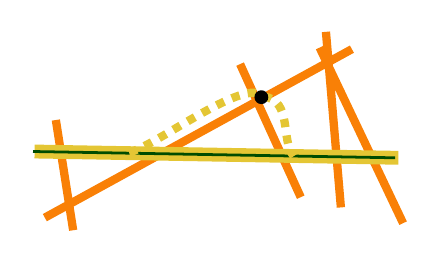
\begin{tikzpicture}[x=1cm,y=1cm]
\draw[orange!90!brown,line width=3pt] (-2.1,-.74)--(1.8,1.40) (-1.96,.50)--(-1.74,-.90) (.38,1.21)--(1.15,-.48) (1.39,1.42)--(2.45,-.81) (1.47,1.62)--(1.66,-.61);
\draw[yellow!55!brown,line width=5pt] (-2.23,.10)--(2.39,.02);
\draw[green!30!black,line width=1pt] (-2.25,.10)--(2.35,.02);
\draw[yellow!55!brown,line width=3pt,dashed] (-1.03,.09) .. controls(-.7,.16) and(.45,1.06)..(.68,.80) .. controls(1.05,.74) and (.89,.25)..(1.06,.04);
\fill (.65,.79) circle(2.5pt);
\end{tikzpicture}}

Revenant à une p.r. $D$ sous-stable passant par $a\in S$, on peut considérer que \deleted{\unsure{les}} (si $\widetilde D$ désigne le rev. des vis) un couloir de spécialisation correspond à un \uline{arc ouvert} de $\widetilde D$, d'extrémités les deux sommets $a',a''$ de $\widetilde D$ au-dessus de $a$. \deleted{En identifiant} \deleted{De façon} Ainsi on peut dire que \deleted{les générisations et} spécialisations de $D$ sont données par des arcs ouverts de $\widetilde D\setminus\{a',a''\}$, mutuellement disjoints, donc contenus dans l'une ou l'autre comp. conn. $\widetilde D_1,\widetilde D_2$ de $\widetilde D\setminus\{a',a''\}$. \deleted{Il y en a}\inserted{Ainsi}, on voit qu'elles forment une \unsure{structuration polygonale des arcs} ``$a',a''$'', et comme sur $\widetilde D_1,\widetilde D_2$ il y a au moins un arc de spécialisation, on voit que le nb total de sommets du polygône de spécialisation-générisation est au moins égal à quatre. \deleted{\unsure{C'est}}

\uline{Ainsi} Dans le graphe \inserted{strict orienté} $\Gamma(\underline\Sigma)$ (où on n'oubliera pas comme sommets les p.r. supercritiques), \deleted{\unsure{chacun des arêtes}}\inserted{pour tt sommet $D$}, l'ens des \deleted{arêtes} arcs qui en sortent $(\simeq\operatorname{Spec}_0(D)\amalg\operatorname{Gen}_0(D))$ est de cardinal au moins $3$ (et au moins $4$ si $D$ n'est pas stable \inserted{i.e. admet une générisation}). Il est muni d'une structure polygonale \inserted{naturelle}, dont l'ens des orientations est \inserted{can. isom. à} l'ens des orientations de $D$. Pour tt flè. de spécialisation \inserted{$D\longrightarrow D'$}, on trouve une iso. can. entre $\omega(D)$ et $\omega(D')$.

[NB L'ens des générisations \inserted{$\operatorname{Gen}_0(D)$} \inserted{de $D$} s'identifie à l'image \deleted{des} inverse de $D\cap S$ dans $\widetilde D$, où pour $D$ non supercritique, $\widetilde D$ désigne le rev. des vis, et pour $D$ supercritique, le rev. image inverse dans $\widetilde X$. Toute flèche

\margin{15}
